\pagenumbering{gobble}

\begin{figure}[!htb]
\minipage{0.32\textwidth}
  
\includegraphics[width=\linewidth]{su}
\endminipage\hfill
\minipage{0.32\textwidth}
  
\includegraphics[width=\linewidth]{iap}
\endminipage\hfill
\minipage{0.32\textwidth}%
  
\includegraphics[width=\linewidth]{cnrs}
\endminipage
\end{figure}

\begin{center}

{\LARGE \textsc{Université Paris-Diderot}}

\vspace{1cm}

{\LARGE \textsc{The Afterglow of the August 17\sp{th} 2017 Binary Neutron Star Merger Multi-messenger Event}}

\vspace{1cm}

\begin{figure}[!htb]
\minipage{0.32\textwidth}
  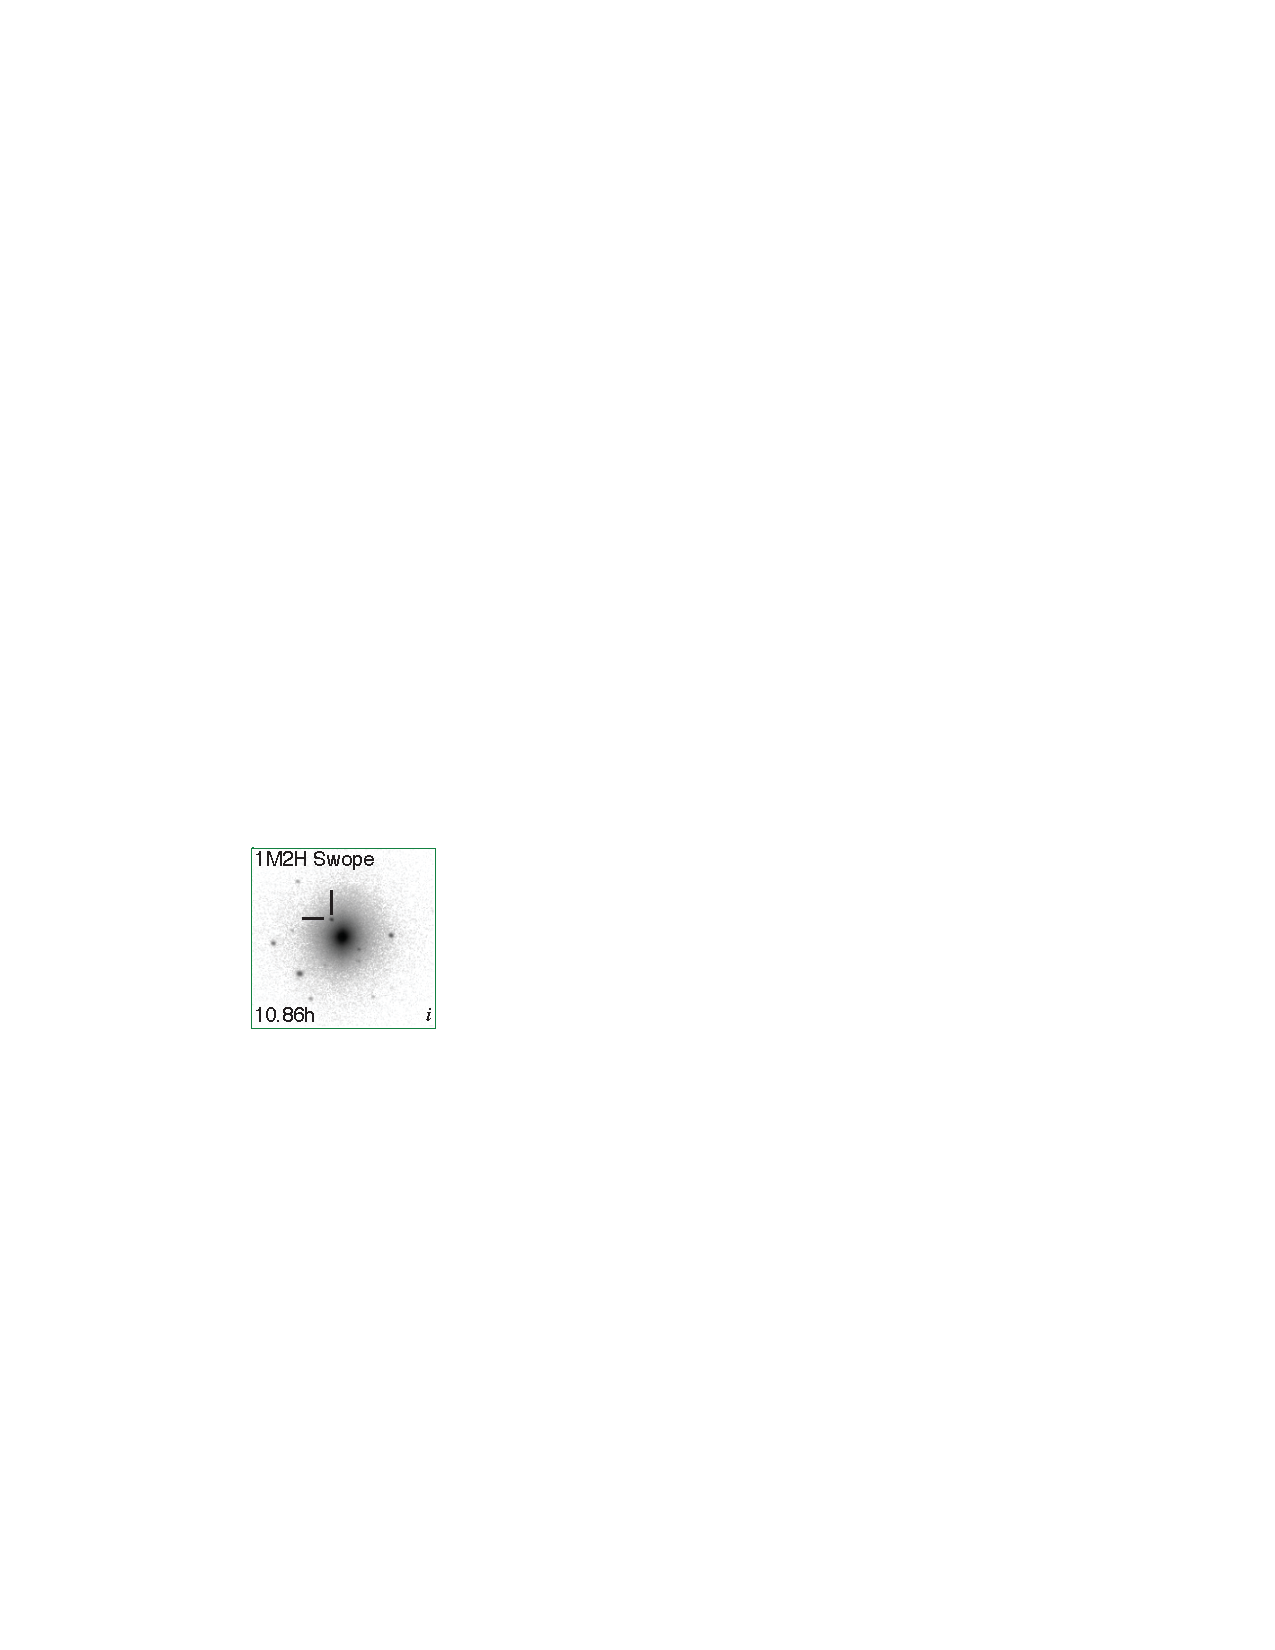
\includegraphics[width=\linewidth]{swope}
\endminipage\hfill
\minipage{0.32\textwidth}
  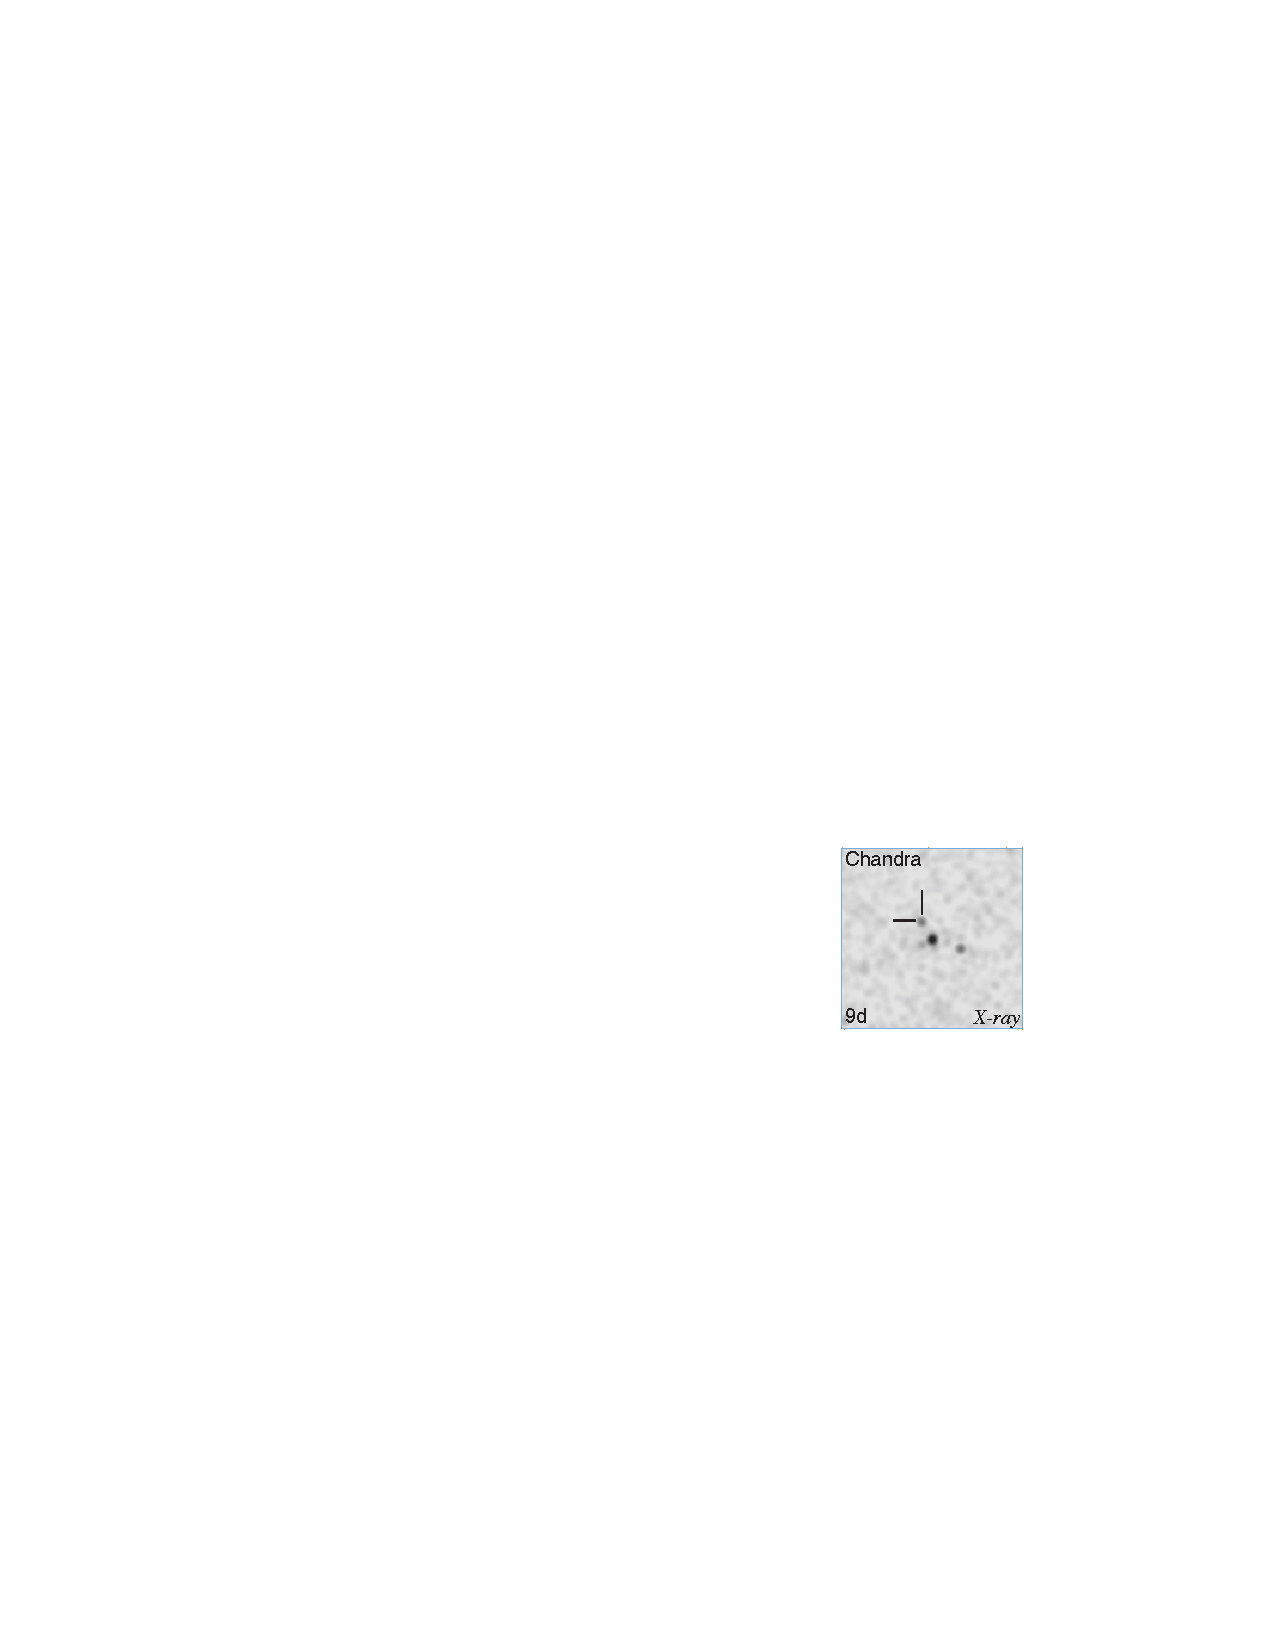
\includegraphics[width=\linewidth]{chandra}
\endminipage\hfill
\minipage{0.32\textwidth}%
  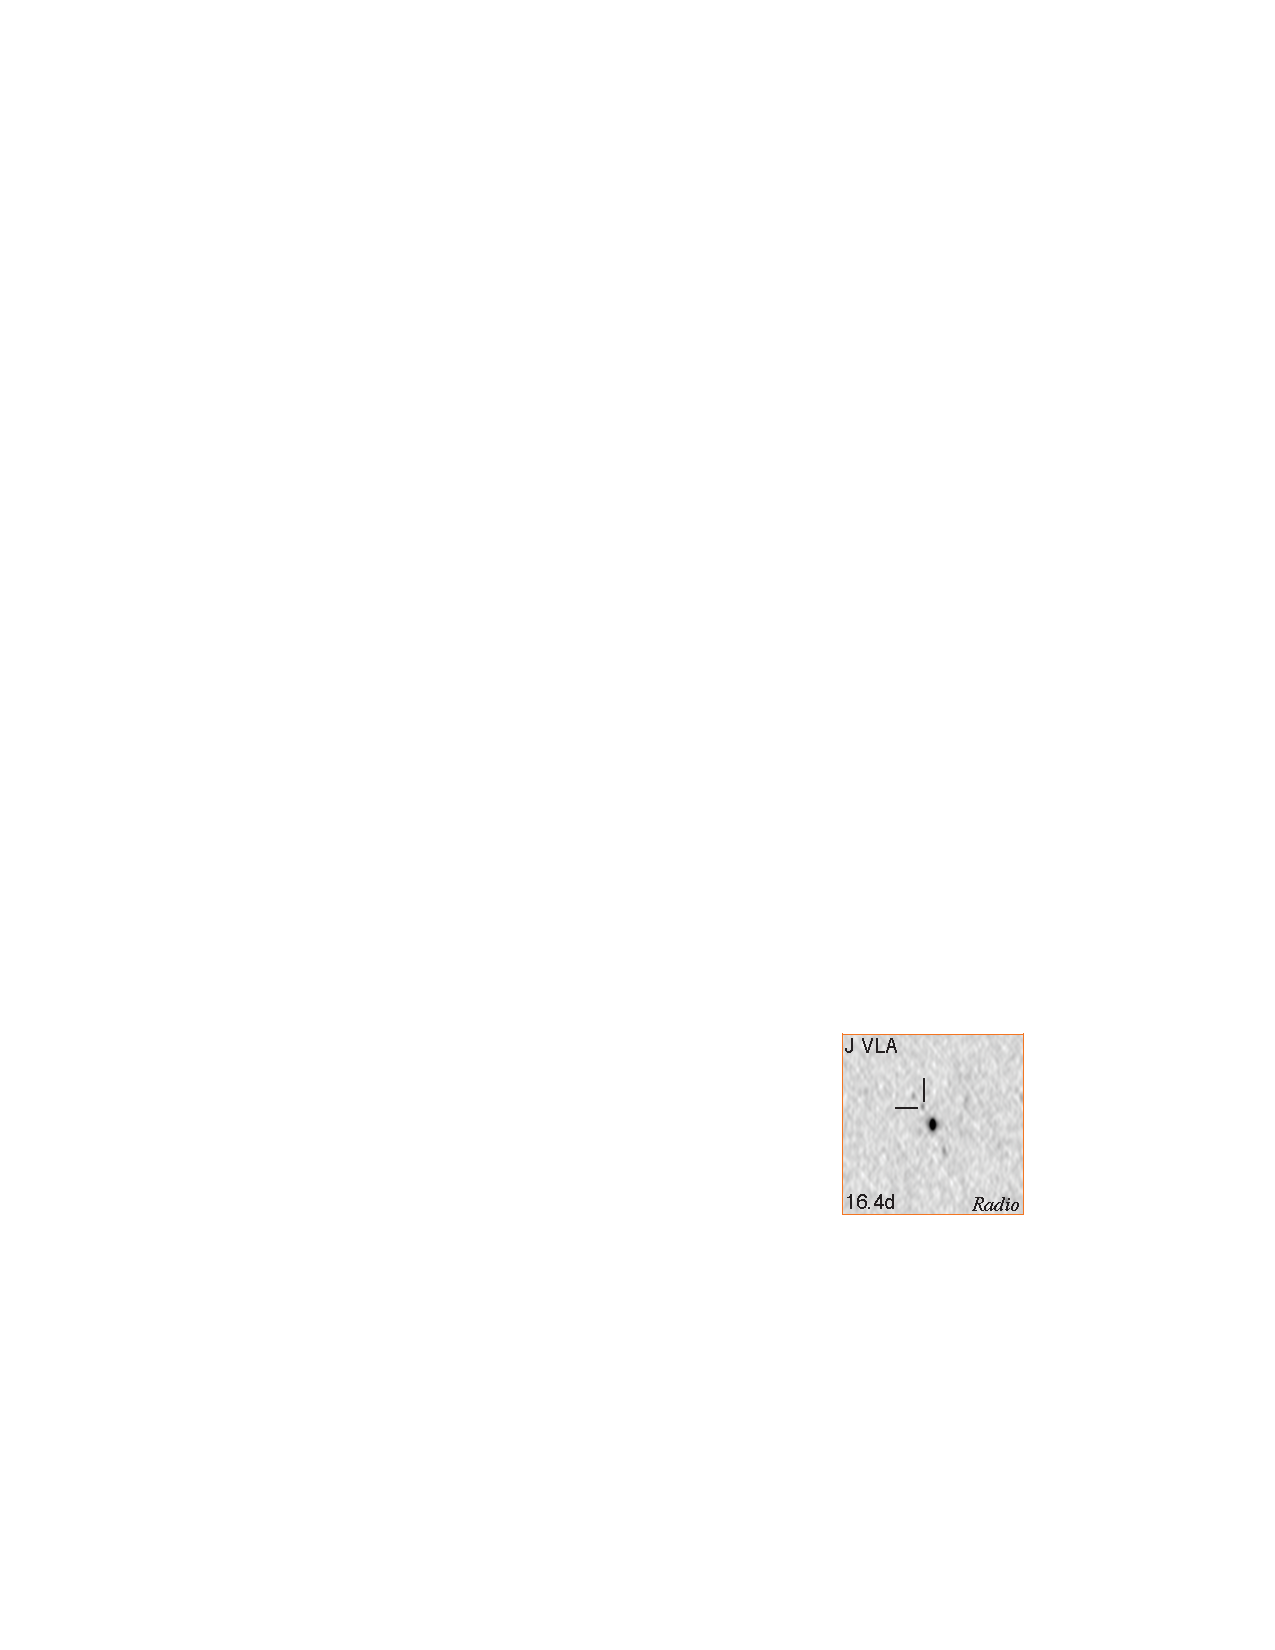
\includegraphics[width=\linewidth]{vla}
\endminipage
\end{figure}
\vspace{2cm}

\begin{tabular}{p{0.7cm}p{3cm}p{3cm}p{5cm}p{5cm}}
\textsc{By:} & \textsc{Raphaël Duque} & & \textsc{Under the supervision of:} & \textsc{Frédéric Daigne} \\
             &                        & &                                   & \& \textsc{Robert Mochkovitch}
\end{tabular}
\vfill

\textsc{April -- June 2018}
\end{center}

\newpage

\quad
\vfill

Cover page illustration credits: \citep[][Fig. 2]{51}.

\newpage

\pagenumbering{roman}
\section*{Summary}

On August 17\sp{th} 2017, gravitational waves from the inspiral phase of a binary neutron star merger were detected for the first time by the LIGO-Virgo network of gravitational interferometers. The source of this signal was aptly triangulated to a 3D error box in a range of distances near 40~Mpc. With a slight delay, a weak short gamma ray burst GRB170817A was detected. Its source was triangulated to a position consistent with the gravitational wave error box. Follow-up ground-based searches inside the gravitational wave inferred region promptly found an optical transient --~the first observed kilonova~-- in the spheroidal galaxy NGC4993. Later, at the position of this optical transient was discovered an afterglow emission, successively in the X-ray, radio and finally optical bands. This afterglow likely originates from shock-accelerated electrons during the deceleration by the external medium of matter ejected from the merger event. We modelize the synchrotron radiation from this shock and explore the radio light curves which would have arisen for a distant observer from various shock geometries and dynamical structures. We find observations to be most consistent with a near-spherical shock, arising from matter ejected with a small range of mildly relativistic ($\Gamma~\sim~2-3$) velocities, and expanding in a rarefied medium of number density $\sim$~10\sp{--3}~cm\sp{--3}. This estimate is in full agreement with densities expected in early-type galaxies. Also, we explore the possibility that a relativistic jet was produced during the merger event. Arguing on the non-observation of a jet-geometry-induced afterglow in the radio data, we constrain any eventual jet's isotropic-equivalent kinetic energy to being less than 10\sp{52}~erg for opening angles larger than 20~deg. In the hypothesis where GRB170817A was produced by a relativistic jet the afterglow of which was not observed, this constraint on jets implies that the gamma-ray efficiency of GRB170817A was at least 0.1\%. Finally, prospects for observation and modeling of binary neutron star mergers are given. In the next observing run (O3) of the LIGO-Virgo network, we expect $10^{+20}_{-8}$ gravitational wave detections from binary neutron star merger events with a kilonova counterpart. Rates on coincident gamma ray bursts are more delicate to obtain.

\vfill

\section*{Résumé}

Le 17 août 2017, les ondes gravitationnelles de la phase spiralante d'une coalescence d'une binaire d'étoiles à neutrons ont été détectées pour la première fois par le réseau d'interféromètres gravitationnels de la collaboration LIGO-Virgo. La source de ce signal a été placée par triangulation dans une région tridimensionnelle de l'espace à une distance de 40~Mpc. Avec un léger retard, un sursaut gamma court faible GRB170817A était détecté. Sa source fut également triangulée, à une position en accord avec la région indiquée par les ondes gravitationnelles. Des recherches de contreparties depuis le sol ont été  entreprises, et une source transitoire optique, une kilonova, a été trouvée dans la galaxie elliptique NGC4993. Plus tard, à la même position que cette source transitoire, une émission rémanente fut détectée, successivement dans les bandes X, radio et ensuite optique. Cette rémanence émane d'une population d'électrons accélérés dans un choc formé par de la matière éjectée lors du phénomène de coalescence, et décélérant au contact du milieu extérieur. Nous avons modélisé le rayonnement synchrotron de cette population d'électrons et calculé les courbes de lumières produites par ce rayonnement pour un observateur distant selon différentes géométries et structures dynamiques du choc. Nous trouvons que les données radio sont le mieux expliquées par un choc quasi-sphérique, formé de matière éjectée avec des vitesses non-uniformes faiblement relativistes ($\Gamma~\sim~2-3$), et en expansion dans un milieu raréfié, de densité numérique $\sim~10^{-3}$~cm\sp{--3}. Cette estimation de densité est en bon accord avec celles attendues dans les galaxies elliptiques telles que NGC4993. Par ailleurs, nous étudions la possibilité qu'un jet relativiste ait été produit lors de l'événement. Se fondant sur la non-observation d'une émission rémanente d'une structure en forme de jet, nous arrivons à contraindre l'énergie cinétique qui doit être inférieure par 10\sp{52}~erg pour un quelconque jet d'angle d'ouverture plus grand que 20~deg. Dans l'hypothèse où GRB170817A a été produit par un jet, cette contrainte correspond à une efficacité de la dissipation en rayons gamma dans GRB170817A qui doit être supérieure à 0.1\%. Enfin, nous ouvrons sur les observations et la modélisation futures des événements de coalescence de binaires d'étoiles à neutrons. Pendant la prochaine phase d'observation du réseau LIGO-Virgo (O3), nous prévoyons $10^{+20}_{-8}$ détections d'ondes gravitationnelles de ces événements avec une kilonova en contrepartie optique. De telles prévisions pour des sursauts gamma sont plus délicates à établir.
\newpage

\newpage

\section*{Acknowledgments}

I am most grateful to my supervisors Robert Mochkovitch and Frédéric Daigne for having opened the doors of the Institut d'Astrophysique de Paris and shown me to the gamma ray burst and more generally the high energy astrophysics community. We will shortly commence a years-long journey among neutron star mergers and multi-wavelength observations, and I look forward to our collaboration. I cannot yet imagine the discoveries to come and what the Universe will give us to contemplate together.

I would also like to thank Jesse Palmerio and Sergei Balashev for their invaluable support all along these months on many topics --~not only astrophysical. I thank Jesse for advice on the graphical content of this document and Sergei for his kind proof-reading.

Finally, none of this work would have so succeeded without the unconditional support, both psychological and spiritual, of Joséphine. I reckon this work as the yield of the efforts of many, you inclusive.


\vspace{3cm}

\begin{flushright}
    \it{l'espace est silence}

    \it{silence comme le frai abondant tombant lentement dans une eau calme}

    H. Michaux
\end{flushright}
